\section{Constructing the queuing model}\label{sec:model}

Owing to a lack of available data on the system and its patients, the options
for the queuing model used are limited compared to those employed in some modern
works. However, there is a precedent for simplifying healthcare systems to a
single node with parallel servers that emulate resource
availability.~\cite{Steins2013}~and~\cite{Williams2015} provide good examples of
how this approach, when paired with discrete event simulation, can expose the
resource needs of a system beyond deterministic queuing theory models. In
particular,~\cite{Williams2015} shows how a single node, multiple server queue
can be used to accurately predict bed capacity and length of stay distributions
in a critical care unit using administrative data.

Following in the suit of recent literature, a single node using a \(M/M/c\)
queue is employed to model a hypothetical ward of patients presenting COPD.\ In
addition to this, the grouping found in Section~\ref{subsec:overview} provides
a set of patient classes in the queue. Under this model, the following
assumptions are made:
\begin{enumerate}
    \item Inter-arrival and service times of patients are each exponentially
        distributed with some mean. This is in spite of the system time
        distributions shown in Figure~\ref{fig:cluster_los} in order to
        simplify the model parameterisation.
    \item There are \(c \in \mathbb{N}\) servers available to arriving patients
        at the node representing the overall resource availability including bed
        capacity and hospital staff.
    \item There is no queue or system capacity. In~\cite{Williams2015}, a
        queue capacity of zero is set under the assumption that any surplus
        arrivals would be sent to another suitable ward or unit. As this
        hypothetical ward represents COPD patients potentially throughout a
        hospital, this assumption is not held.
    \item Without the availability of expert clinical knowledge, a first-in
        first-out service policy is employed in lieu of some patient priority 
        framework.
\end{enumerate}

Each group of patients has its own arrival distribution. The parameter of this
distribution is taken to be the reciprocal of the mean inter-arrival times for
that group and is denoted by \(\lambda_i\) for each cluster \(i\).

Like arrivals, each group of patients has its own service time distribution.
Without full details of the process order or idle periods during a spell, some
assumption must be made about the true `service' time of a patient in hospital.
It is assumed here that the mean service time of a group of patients may be
approximated via their mean length of stay, i.e.\ the mean time spent in the
system. For simplicity, this work assumes that for each cluster, \(i\), the mean
service time of that cluster, \(\frac{1}{\mu_i}\), is directly proportional
to the mean total system time of that cluster, \(\frac{1}{\phi_i}\), such that:
\begin{equation}\label{eq:services}
    \mu_i = p_i \phi_i
\end{equation}

\noindent where \(p_i \in \interval[open left]{0}{1}\) is some parameter to be
determined for each group.

One of the few ground truths available in the provided data is the distribution
of the total length of stay. Given that the length of stay and resource
availability are connected, the approach here will be to simulate the length of
stay distribution for a range of values \(p_i\) and \(c\) in order to find the
parameters that best match the observed data.

The statistical comparison of two or more distributions can be done in a number
of ways. Such methods include the Kolmogorov-Smirnov test, a variety of
discrepancy approaches such as summed mean-squared error, and \(f\)-divergences.
A popular choice amongst the latter group (which may be considered
distance-like) is the Kullback-Leibler divergence which measures relative
information entropy from one probability distribution to
another~\cite{Kullback1951}. The key issue with many of these methods is that
they lack interpretability which is paramount when conveying information to
stakeholders. Interpretability not just from explaining how something works but
how its results may be explained also.

As such, a reasonable candidate is the (first) Wasserstein metric, also known as
the `earth mover' or `digger' distance~\cite{Vaserstein1969}. The Wasserstein
metric satisfies the conditions of a formal mathematical metric (like the
typical Euclidean distance), and its values take the units of the distributions
under comparison (in this case: days). Both of these characteristics can aid
understanding and explanation. In simple terms, the distance measures the
approximate `minimal work' required to move between two probability
distributions where `work' can be loosely defined as the product of how much of
the distribution's mass is to be moved and the distance it must be moved
by. More formally, the Wasserstein distance between two probability
distributions \(U\) and \(V\) is defined as:
\begin{equation}\label{eq:wasserstein}
    W(U, V) = \int_{0}^{1} \left\vert F^{-1}(t) - G^{-1}(t) \right\vert dt
\end{equation}

\noindent where \(F\) and \(G\) are the cumulative density functions of \(U\)
and \(V\) respectively. A proof of~\eqref{eq:wasserstein} is presented
in~\cite{Ramdas2017}. The parameter set with the smallest maximum distance
between any cluster's simulated system time distribution and the overall
observed length of stay distribution is then taken to be the most appropriate.
To be specific, let \(T\) denote the system time distribution of all of
the observed data and let \(T_{i,c,p}\) denote the system time distribution for
cluster \(i\) obtained from a simulation with \(c\) servers and
\(p := \left(p_0, p_1, p_2, p_3\right)\). Then the optimal parameter set
\(\left(c^*, p^*\right)\) is given by:
\begin{equation}\label{eq:parameters}
    \left(c^*, p^*\right) = \argmin_{c, p} \left\{%
        \max_{i} \left\{ W\left(T_{i,c,p}, T\right) \right\}%
    \right\}
\end{equation}

\begin{figure}
    \resizebox{\imgwidth}{!}{%
        \includestandalone{tex/process}
    }
    \caption{%
        A diagrammatic depiction of the queuing parameter recovery process.
    }\label{fig:process}
\end{figure}

The parameter sweep included values of each \(p_i\) from \(0.5\)
to \(1.0\) with a granularity of \(5.0 \times 10^{-2}\) and values of \(c\) from
\(40\) to \(60\) at steps of \(5\).  These choices were informed by the
assumptions of the model and formative analysis to reduce the parameter space
given the computational resources required to conduct the simulations. Each
parameter set was repeated \(50\) times with each simulation running for four
years of virtual time. The warm-up and cool-down periods were taken to be
approximately one year each leaving two years of simulated data from each
repetition.

\begin{figure}
    \centering%
    \begin{subfigure}{.5\imgwidth}
        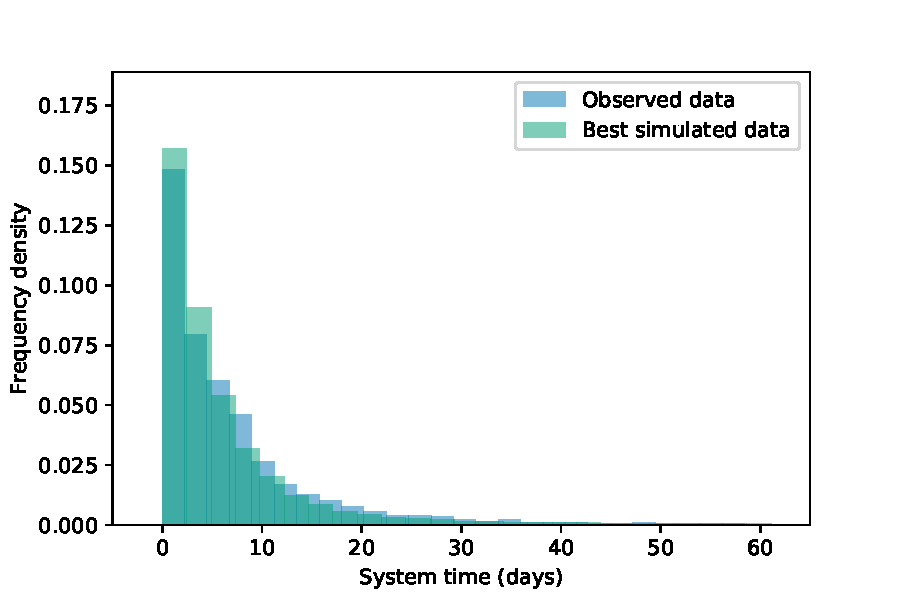
\includegraphics[width=\linewidth]{best_params}
        \caption{}\label{fig:best_params}
    \end{subfigure}\hfill%
    \begin{subfigure}{.5\imgwidth}
        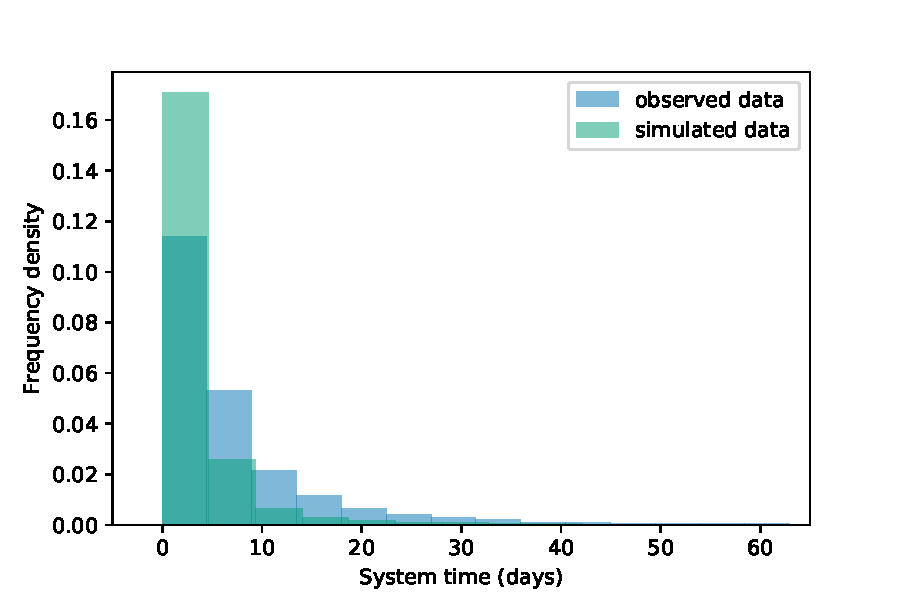
\includegraphics[width=\linewidth]{worst_params}
        \caption{}\label{fig:worst_params}
    \end{subfigure}
    \caption{Histograms of the simulated and observed length of stay data for
             the (\subref{fig:best_params}) best and (\subref{fig:worst_params})
             worst parameter sets.}\label{fig:params}
\end{figure}

The results of this parameter sweep can be summarised in
Figure~\ref{fig:params}. Each plot shows a comparison of the observed lengths
of stay across all groups and the newly simulated data with the best and worst
parameter sets respectively. It can be seen that, in the best case, a very close
fit has been found. Meanwhile, Figure~\ref{fig:worst_params} highlights the
importance of good parameter estimation under this model since the likelihood of
short-stay patient arrivals has been inflated disproportionately against the
tail of the distribution. Table~\ref{tab:comparison} reinforces these results
numerically, showing a clear fit by the best parameters across the board.

\begin{table}
    \centering
    \resizebox{\tabwidth}{!}{\begin{tabular}{lrrrrrrrrrrrrr}
\toprule
{} & \multicolumn{6}{l}{Model parameter and result} & \multicolumn{7}{l}{LOS statistic} \\
{} &                    \(p_0\) & \(p_1\) & \(p_2\) & \(p_3\) & \(c\) & Max. distance &          Mean &   Std. &  Min. &   25\% &  Med. &   75\% &    Max. \\
\midrule
Observed        &                        NaN &     NaN &     NaN &     NaN &   NaN &          0.00 &          7.70 &  11.86 & -0.02 &  1.49 &  4.20 &  8.93 &  224.93 \\
Best simulated  &                        1.0 &     1.0 &     1.0 &     0.5 &  50.0 &          1.30 &          7.11 &  12.41 &  0.00 &  1.44 &  3.55 &  7.64 &  244.46 \\
Worst simulated &                        0.5 &     0.5 &     0.5 &     1.0 &  40.0 &          4.25 &          4.36 &  13.40 &  0.00 &  0.72 &  1.78 &  3.84 &  463.01 \\
\bottomrule
\end{tabular}
}
    \caption{A comparison of the observed data, and the best and worst simulated
        data based on the model parameters and summary statistics for length of
    stay (LOS).}\label{tab:comparison}
\end{table}

In this section, the clustering has been used to enrich the overall queuing
model and to recover the parameters for several classes within that queue to a
high standard. Now, using this model, the next section conducts an investigation
into the underlying system by adjusting the parameters of the queue with the
clustering.
